% This file was created with tikzplotlib v0.10.1.
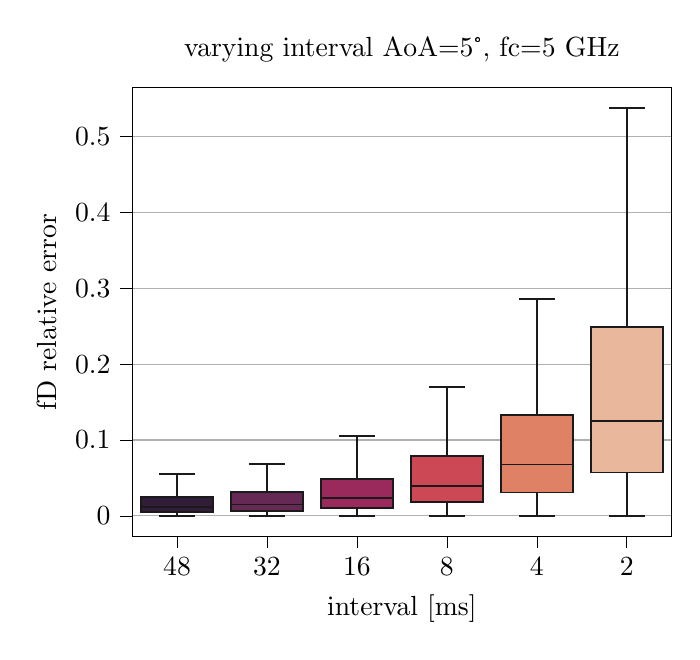
\begin{tikzpicture}

\definecolor{black26}{RGB}{26,26,26}
\definecolor{brown1544291}{RGB}{154,42,91}
\definecolor{burlywood233183155}{RGB}{233,183,155}
\definecolor{darkgray176}{RGB}{176,176,176}
\definecolor{darkslategray1014183}{RGB}{101,41,83}
\definecolor{darkslategray502957}{RGB}{50,29,57}
\definecolor{indianred2037284}{RGB}{203,72,84}
\definecolor{salmon222129101}{RGB}{222,129,101}

\begin{axis}[
tick align=outside,
tick pos=left,
title={varying interval AoA=5°, fc=5 GHz},
x grid style={darkgray176},
xlabel={interval [ms]},
xmin=-0.5, xmax=5.5,
xtick style={color=black},
xtick={0,1,2,3,4,5},
xticklabels={48,32,16,8,4,2},
y grid style={darkgray176},
ylabel={fD relative error},
ymajorgrids,
ymin=-0.0268805384380875, ymax=0.564498828079264,
ytick style={color=black}
]
\path [draw=black26, fill=darkslategray502957, semithick]
(axis cs:-0.4,0.00494735586188221)
--(axis cs:0.4,0.00494735586188221)
--(axis cs:0.4,0.0252206813995251)
--(axis cs:-0.4,0.0252206813995251)
--(axis cs:-0.4,0.00494735586188221)
--cycle;
\path [draw=black26, fill=darkslategray1014183, semithick]
(axis cs:0.6,0.00650007256249933)
--(axis cs:1.4,0.00650007256249933)
--(axis cs:1.4,0.0311303726953379)
--(axis cs:0.6,0.0311303726953379)
--(axis cs:0.6,0.00650007256249933)
--cycle;
\path [draw=black26, fill=brown1544291, semithick]
(axis cs:1.6,0.0105471194385272)
--(axis cs:2.4,0.0105471194385272)
--(axis cs:2.4,0.0484905288507537)
--(axis cs:1.6,0.0484905288507537)
--(axis cs:1.6,0.0105471194385272)
--cycle;
\path [draw=black26, fill=indianred2037284, semithick]
(axis cs:2.6,0.0179300402829651)
--(axis cs:3.4,0.0179300402829651)
--(axis cs:3.4,0.0789394706158319)
--(axis cs:2.6,0.0789394706158319)
--(axis cs:2.6,0.0179300402829651)
--cycle;
\path [draw=black26, fill=salmon222129101, semithick]
(axis cs:3.6,0.0306717154370697)
--(axis cs:4.4,0.0306717154370697)
--(axis cs:4.4,0.132897447241021)
--(axis cs:3.6,0.132897447241021)
--(axis cs:3.6,0.0306717154370697)
--cycle;
\path [draw=black26, fill=burlywood233183155, semithick]
(axis cs:4.6,0.0572945244113831)
--(axis cs:5.4,0.0572945244113831)
--(axis cs:5.4,0.249466889208918)
--(axis cs:4.6,0.249466889208918)
--(axis cs:4.6,0.0572945244113831)
--cycle;
\addplot [semithick, black26]
table {%
0 0.00494735586188221
0 2.02120740608642e-06
};
\addplot [semithick, black26]
table {%
0 0.0252206813995251
0 0.0555602199674846
};
\addplot [semithick, black26]
table {%
-0.2 2.02120740608642e-06
0.2 2.02120740608642e-06
};
\addplot [semithick, black26]
table {%
-0.2 0.0555602199674846
0.2 0.0555602199674846
};
\addplot [semithick, black26]
table {%
1 0.00650007256249933
1 3.41858155715185e-07
};
\addplot [semithick, black26]
table {%
1 0.0311303726953379
1 0.0680333841190556
};
\addplot [semithick, black26]
table {%
0.8 3.41858155715185e-07
1.2 3.41858155715185e-07
};
\addplot [semithick, black26]
table {%
0.8 0.0680333841190556
1.2 0.0680333841190556
};
\addplot [semithick, black26]
table {%
2 0.0105471194385272
2 7.30401557308843e-07
};
\addplot [semithick, black26]
table {%
2 0.0484905288507537
2 0.105264307286387
};
\addplot [semithick, black26]
table {%
1.8 7.30401557308843e-07
2.2 7.30401557308843e-07
};
\addplot [semithick, black26]
table {%
1.8 0.105264307286387
2.2 0.105264307286387
};
\addplot [semithick, black26]
table {%
3 0.0179300402829651
3 1.92069749176969e-06
};
\addplot [semithick, black26]
table {%
3 0.0789394706158319
3 0.170179448544785
};
\addplot [semithick, black26]
table {%
2.8 1.92069749176969e-06
3.2 1.92069749176969e-06
};
\addplot [semithick, black26]
table {%
2.8 0.170179448544785
3.2 0.170179448544785
};
\addplot [semithick, black26]
table {%
4 0.0306717154370697
4 1.10258406899782e-06
};
\addplot [semithick, black26]
table {%
4 0.132897447241021
4 0.286168524572987
};
\addplot [semithick, black26]
table {%
3.8 1.10258406899782e-06
4.2 1.10258406899782e-06
};
\addplot [semithick, black26]
table {%
3.8 0.286168524572987
4.2 0.286168524572987
};
\addplot [semithick, black26]
table {%
5 0.0572945244113831
5 8.74184596314485e-06
};
\addplot [semithick, black26]
table {%
5 0.249466889208918
5 0.537617947783021
};
\addplot [semithick, black26]
table {%
4.8 8.74184596314485e-06
5.2 8.74184596314485e-06
};
\addplot [semithick, black26]
table {%
4.8 0.537617947783021
5.2 0.537617947783021
};
\addplot [semithick, black26]
table {%
-0.4 0.0116679228660671
0.4 0.0116679228660671
};
\addplot [semithick, black26]
table {%
0.6 0.0148986886045227
1.4 0.0148986886045227
};
\addplot [semithick, black26]
table {%
1.6 0.0238620424058169
2.4 0.0238620424058169
};
\addplot [semithick, black26]
table {%
2.6 0.039243781006004
3.4 0.039243781006004
};
\addplot [semithick, black26]
table {%
3.6 0.0677608944539392
4.4 0.0677608944539392
};
\addplot [semithick, black26]
table {%
4.6 0.124714883703833
5.4 0.124714883703833
};
\end{axis}

\end{tikzpicture}
